\chapter{Advanced Features of \textsc{Larkita}}

\begin{figure}[h]
  \centering
    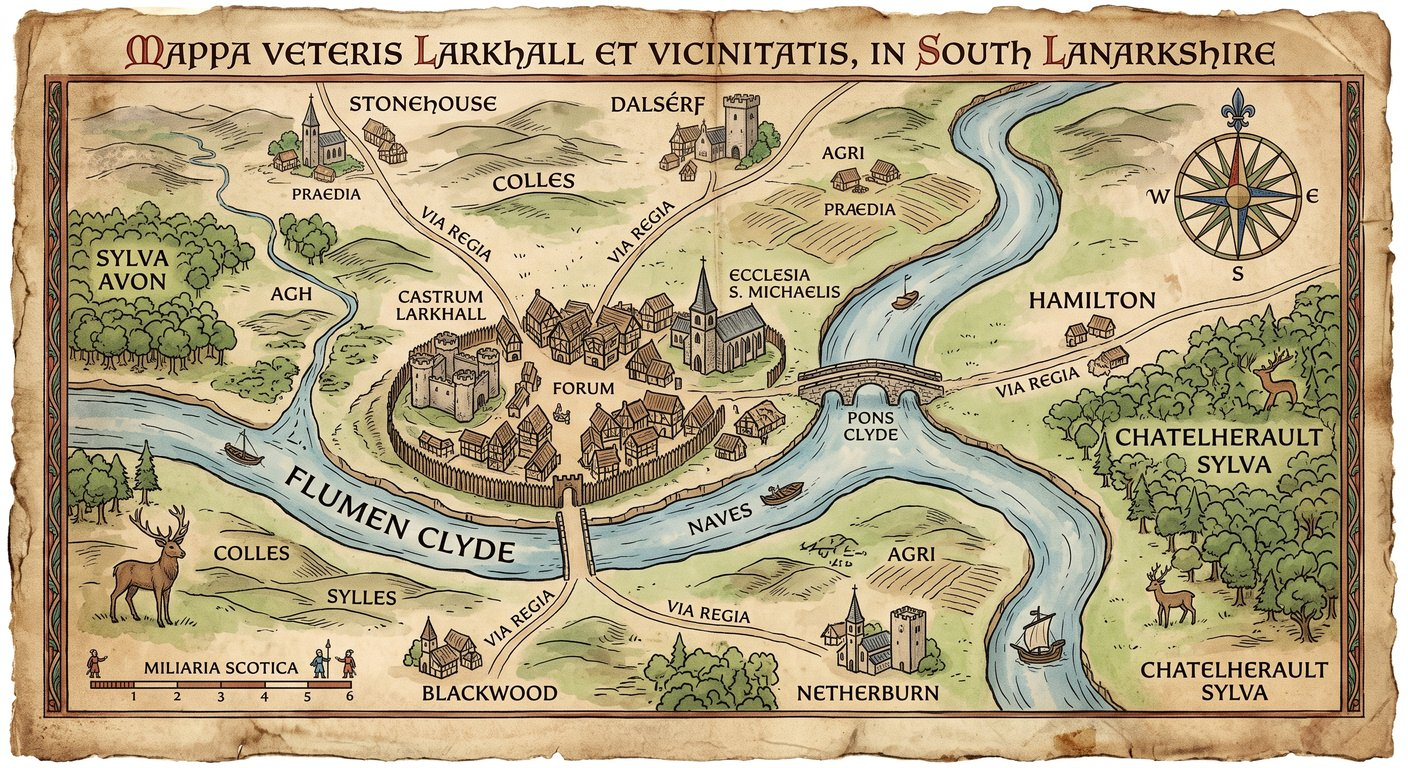
\includegraphics[width=17cm]{Abbildungen/larkhall.jpg}
  \caption{Larkhall in South Lanarkshire, Scotland.}
  \label{fig:larkhall.jpg}
  \end{figure}

When we discussed the parser generator \simtextsc{Larkita} in chapter 7, we were not able to discuss all the
features of \simtextsc{Larkita}, since the underlying theory, which is the theory of LR parsing, had not been
developed.  Since we have acquainted ourselves with this theory in the previous chapter, we are finally able to
discuss some of the more advanced features of \simtextsc{Larkita}.
\begin{enumerate}
\item First, we show how shift-reduce and reduce-reduce conflicts are reported by \simtextsc{Larkita} and how the
      states of the canonical LR(1) parser that \simtextsc{Larkita} computes can be inspected.
\item Then we discuss how these conflicts can be resolved.  As \simtextsc{Larkita} resolves every shift-reduce
      conflict in favour of shifting and offers no way to change this decision, the precedences and
      associativities of the operators have to be encoded into the grammar itself.
\item Finally, we see that \simtextsc{Larkita} has no problem with a grammar that is an LR(1) grammar but not an
      \simtextsc{Lalr}(1) grammar, and we show how \simtextsc{Larkita} can reduce the number of states by merging
      those states that can be merged safely.
\end{enumerate}
All examples of this chapter are available as Jupyter notebooks in the following directory:
\\[0.2cm]
\hspace*{1.3cm}
\href{https://github.com/karlstroetmann/Formal-Languages/blob/master/Python/Chapter-11}{\texttt{Python/Chapter-11}}.
\vspace*{-0.2cm}

\begin{center}
  \begin{tabular}[t]{|l|p{0.45\textwidth}|}
    \hline
    notebook & topic \\
    \hline
    \hline
    \href{https://github.com/karlstroetmann/Formal-Languages/blob/master/Python/Chapter-11/01-Conflicts.ipynb}{\texttt{01-Conflicts.ipynb}}            & shift-reduce conflicts and how to inspect the states \\
    \hline
    \href{https://github.com/karlstroetmann/Formal-Languages/blob/master/Python/Chapter-11/02-Conflicts-Resolved.ipynb}{\texttt{02-Conflicts-Resolved.ipynb}}   & encoding operator precedences into the grammar       \\
    \hline
    \href{https://github.com/karlstroetmann/Formal-Languages/blob/master/Python/Chapter-11/03-Look-Ahead.ipynb}{\texttt{03-Look-Ahead.ipynb}}           & a reduce-reduce conflict caused by insufficient look-ahead \\
    \hline
    \href{https://github.com/karlstroetmann/Formal-Languages/blob/master/Python/Chapter-11/04-Look-Ahead-Solved.ipynb}{\texttt{04-Look-Ahead-Solved.ipynb}}    & the same grammar, rewritten so that it is LR(1) \\
    \hline
    \href{https://github.com/karlstroetmann/Formal-Languages/blob/master/Python/Chapter-11/05-Mysterious-Conflicts.ipynb}{\texttt{05-Mysterious-Conflicts.ipynb}} & a grammar that is LR(1), but not \simtextsc{Lalr}(1) \\
    \hline
    \href{https://github.com/karlstroetmann/Formal-Languages/blob/master/Python/Chapter-11/06-Merging-States.ipynb}{\texttt{06-Merging-States.ipynb}} & merging states with the same core \\
    \hline
  \end{tabular}
\end{center}

\section{Shift-Reduce and Reduce-Reduce Conflicts}
In this section we show how shift-reduce and reduce-reduce conflicts are dealt with in \simtextsc{Larkita}.
Figure \ref{fig:Conflicts.ipynb} on page \pageref{fig:Conflicts.ipynb} shows a grammar for arithmetical
expressions that is ambiguous because it does not specify the precedence of the different arithmetical
operators.

\begin{figure}[!ht]
\centering
\begin{minted}[ frame        = lines,
                framesep     = 0.3cm,
                bgcolor      = sepia,
                numbers      = left,
                numbersep    = 0.3cm,
                xleftmargin  = 0.8cm,
                xrightmargin = 0.8cm,
              ]{larkita_lexer.py:LarkitaLexer}
    expr : expr "+" expr
         | expr "*" expr
         | NUMBER

    NUMBER : /0|[1-9][0-9]*/

    %import common.WS
    %ignore WS
\end{minted}
\vspace*{-0.3cm}
\caption{An ambiguous grammar for arithmetical expressions.}
\label{fig:Conflicts.ipynb}
\end{figure}
\FloatBarrier

\noindent
Note that in a \simtextsc{Larkita} grammar the syntactical variables are written in lower case, while the names of
the token classes are written in upper case.  The operators \squoted{+} and \squoted{*} occur as string literals
inside the grammar rules.  As we have seen in Chapter \ref{chapter:ply}, these literals form the heads of the
abstract syntax trees, e.g.~the first alternative yields a tuple of the form \texttt{('+', $\textsl{lhs}$,
$\textsl{rhs}$)}.  The way the abstract syntax tree is built has no influence on the parse table.

This grammar does not specify whether the string
\\[0.2cm]
\hspace*{1.3cm}
``\texttt{1 + 2 * 3}'' \quad is interpreted as \quad  ``\texttt{(1 + 2) * 3}'' \quad or as \quad ``\texttt{1 +
  (2 * 3)}''.
\\[0.2cm]
Since every LR(1) grammar is unambiguous, but the grammar shown in Figure \ref{fig:Conflicts.ipynb} is
ambiguous, it has to have at least one shift-reduce or reduce-reduce conflict.  This grammar is part of the
jupyter notebook
\\[0.2cm]
\hspace*{1.3cm}
\href{https://github.com/karlstroetmann/Formal-Languages/blob/master/Python/Chapter-11/01-Conflicts.ipynb}{Python/Chapter-11/01-Conflicts.ipynb}.
\\[0.2cm]

\subsection{How \textsc{Larkita} Reports Its Conflicts}
\simtextsc{Larkita} reports the conflicts of a grammar in two ways.
\begin{enumerate}
\item If the parse table has shift-reduce conflicts, \simtextsc{Larkita} resolves them in favour of shifting and
      issues a \blue{warning} of the class \texttt{ConflictWarning}.  In a Jupyter notebook, this warning is
      shown below the cell that creates the parser.  A reduce-reduce conflict raises an \blue{exception} of the
      class \texttt{GrammarError}.
\item \simtextsc{Larkita} always writes a description of all states of the parser into an \blue{output
      file}\index{output file (Larkita)@output file (\simtextsc{Larkita})}.  The name of this file is specified by
      the keyword argument \texttt{out\_file}.  Among other things, the section \texttt{Conflicts} of this file
      lists all conflicts.
\end{enumerate}
Figure \ref{fig:conflicts-code} on page \pageref{fig:conflicts-code} shows how the parser for the grammar given
in Figure \ref{fig:Conflicts.ipynb} is created.

\begin{figure}[!ht]
\centering
\begin{minted}[ frame        = lines,
                framesep     = 0.3cm,
                bgcolor      = sepia,
                numbers      = left,
                numbersep    = 0.3cm,
                xleftmargin  = 0.3cm,
                xrightmargin = 0.3cm,
              ]{python3}
    from larkita import Larkita, ConflictWarning, GrammarError

    parser = Larkita(grammar, out_file='conflicts.out')
\end{minted}
\vspace*{-0.3cm}
\caption{Creating a parser.}
\label{fig:conflicts-code}
\end{figure}
\FloatBarrier

\noindent
When we run this code with the grammar of Figure \ref{fig:Conflicts.ipynb}, \simtextsc{Larkita} issues the
warning
\\[0.2cm]
\hspace*{1.3cm}
\texttt{ConflictWarning: 4 shift/reduce conflict(s) were resolved as shift, see conflicts.out}
\\[0.2cm]
and the section \texttt{Conflicts} of the file \texttt{conflicts.out} contains the text that is shown in Figure
\ref{fig:Conflicts.warnings} on page \pageref{fig:Conflicts.warnings}.

\begin{figure}[!ht]
\centering
\begin{minted}[ frame        = lines,
                framesep     = 0.3cm,
                bgcolor      = sepia,
                numbers      = left,
                numbersep    = 0.3cm,
                xleftmargin  = 0.3cm,
                xrightmargin = 0.3cm,
              ]{text}
    State 5, shift/reduce conflict on "+", resolved as shift
        - shift and go to state 3
        - reduce using rule (1) expr → expr "+" expr

    State 5, shift/reduce conflict on "*", resolved as shift
        - shift and go to state 4
        - reduce using rule (1) expr → expr "+" expr

    State 6, shift/reduce conflict on "+", resolved as shift
        - shift and go to state 3
        - reduce using rule (2) expr → expr "*" expr

    State 6, shift/reduce conflict on "*", resolved as shift
        - shift and go to state 4
        - reduce using rule (2) expr → expr "*" expr
\end{minted}
\vspace*{-0.3cm}
\caption{The conflicts reported for the grammar of Figure \ref{fig:Conflicts.ipynb}.}
\label{fig:Conflicts.warnings}
\end{figure}
\FloatBarrier

\noindent
Hence there are four shift-reduce conflicts.  Every one of these entries names
\begin{enumerate}
\item the state $s$ and the terminal $o$ for which the entry $\textsl{action}(s,o)$ of the action table is
      ambiguous,
\item the action that has been chosen, and
\item the alternatives, i.e.~the state that the parser could shift to and the grammar rule $r$ that could have
      been used to reduce the symbol stack in this situation.
\end{enumerate}
The rules are referred to by their numbers in the section \texttt{Rules} at the beginning of the output file.

The important observation is the remark ``\blue{\texttt{resolved as shift}}\index{shift-reduce conflict!resolution by Larkita@resolution by \simtextsc{Larkita}}'': \simtextsc{Larkita} resolves
\emph{every} shift-reduce conflict in favour of shifting.  There is no way to change this decision for an
individual conflict.  The only choice we have is to declare that we do not want to tolerate conflicts at all.
The module \texttt{warnings} of \textsl{Python} can turn the \texttt{ConflictWarning} into an exception, as
shown in Figure \ref{fig:conflicts-strict} on page \pageref{fig:conflicts-strict}.  Then the message of the
exception is the text of the warning.  It is a good idea to develop a grammar this way, for then a conflict
cannot be overlooked.

\begin{figure}[!ht]
\centering
\begin{minted}[ frame        = lines,
                framesep     = 0.3cm,
                bgcolor      = sepia,
                numbers      = left,
                numbersep    = 0.3cm,
                xleftmargin  = 0.3cm,
                xrightmargin = 0.3cm,
              ]{python3}
    import warnings

    with warnings.catch_warnings():
        warnings.simplefilter('error', ConflictWarning)
        try:
            Larkita(grammar, out_file='conflicts.out')
        except ConflictWarning as e:
            print(e)
\end{minted}
\vspace*{-0.3cm}
\caption{Turning shift-reduce conflicts into errors.}
\label{fig:conflicts-strict}
\end{figure}
\FloatBarrier

\noindent
Reduce-reduce conflicts are treated much more severely.  A reduce-reduce conflict always raises an exception of
class \texttt{GrammarError}.  We will see an example of this in Section \ref{section:resolving-conflicts}.

\subsection{Inspecting the LR(1) States}
The section \texttt{States} of the output file describes all states of the canonical LR(1) parser that has been
computed by \simtextsc{Larkita}.  Every state lists its \blue{marked rules} together with their
\blue{follow sets}, i.e.~the tokens that may follow the rule.  A marked rule of the form
$A \rightarrow \alpha \bullet \beta: L$ is written as
\\[0.2cm]
\hspace*{1.3cm}
$A$ \texttt{→} $\alpha$ \texttt{•} $\beta$ \texttt{\{} $L$ \texttt{\}}
\\[0.2cm]
and the marked rules that are added by computing the closure of a state are marked with the character
``\texttt{+}''.  Below the marked rules, the actions and the gotos of the state are listed and, if the state has
conflicts, these conflicts are listed below its actions.

Given the grammar shown in Figure \ref{fig:Conflicts.ipynb}, \simtextsc{Larkita} creates seven different states.
Figure \ref{fig:Conflicts.ipynb:state5} on page \pageref{fig:Conflicts.ipynb:state5} shows the most interesting
of these, together with its actions.

\begin{figure}[!ht]
\centering
\begin{minted}[ frame        = lines,
                framesep     = 0.3cm,
                bgcolor      = sepia,
                numbers      = left,
                numbersep    = 0.3cm,
                xleftmargin  = 0.3cm,
                xrightmargin = 0.3cm,
              ]{text}
    State 5

        (1)  expr → expr • "+" expr  { "*", "+", $END }
        (1)  expr → expr "+" expr •  { "*", "+", $END }
        (2)  expr → expr • "*" expr  { "*", "+", $END }

        "*"   shift and go to state 4
        "+"   shift and go to state 3
        $END  reduce using rule (1) expr → expr "+" expr

        shift/reduce conflict on "+", resolved as shift
            - shift and go to state 3
            - reduce using rule (1) expr → expr "+" expr
        shift/reduce conflict on "*", resolved as shift
            - shift and go to state 4
            - reduce using rule (1) expr → expr "+" expr
\end{minted}
\vspace*{-0.3cm}
\caption{One of the states with a conflict.}
\label{fig:Conflicts.ipynb:state5}
\end{figure}

\noindent
The end of the input is called \texttt{\$END} by \simtextsc{Larkita}.  The state shown in Figure
\ref{fig:Conflicts.ipynb:state5} is reached after an expression of the form
$\textsl{expr}\; \aquoted{+} \;\textsl{expr}$ has been read.  There are two shift-reduce conflicts in this
state: both the token \aquoted{+} and the token \aquoted{*} are elements of the follow set of the marked rule
\\[0.2cm]
\hspace*{1.3cm}
$\textsl{expr} \rightarrow \textsl{expr} \aquoted{+} \textsl{expr} \bullet$,
\\[0.2cm]
so for both of these tokens the parser could either reduce with this rule or shift the operator.  We see that
both conflicts have been decided in favour of shifting: the only reduce action that is left in this state is
the one for the end of input.  The discarded reduce actions are listed below the actions of the state.

Of course, resolving these conflicts in favour of shifting is wrong: the string
\\[0.2cm]
\hspace*{1.3cm}
\texttt{1 * 2 + 3}
\\[0.2cm]
is then interpreted as ``\texttt{1 * (2 + 3)}'' and not as ``\texttt{(1 * 2) + 3}''.  You can convince yourself
of this by inspecting the abstract syntax tree that \simtextsc{Larkita} produces for this string.

\section{Operator Precedence \label{section:operator-precedence}}

\begin{figure}[!ht]
  \begin{center}    
  \framebox{
  \framebox{
    \begin{minipage}[t]{9cm}    
  \begin{eqnarray*}
  \textsl{expr}    & \rightarrow & \;\textsl{expr} \aquoted{+} \textsl{expr}  \\
                   & \mid        & \;\textsl{expr} \aquoted{-} \textsl{expr}  \\
                   & \mid        & \;\textsl{expr} \aquoted{*} \textsl{expr}  \\
                   & \mid        & \;\textsl{expr} \aquoted{/} \textsl{expr}  \\
                   & \mid        & \;\textsl{expr} \aquoted{\symbol{94}} \textsl{expr}  \\
                   & \mid        & \aquoted{(} \textsl{expr} \aquoted{)}       \\
                   & \mid        & \;\simtextsc{Number}                            
  \end{eqnarray*}
  \vspace*{-0.5cm}
  \end{minipage}}}
  \end{center}
  \caption{An ambiguous grammar for arithmetical expressions.}
  \label{fig:grammar-resolved.g}
\end{figure}

\noindent
Consider the grammar for arithmetical expressions shown in Figure \ref{fig:grammar-resolved.g} on page
\pageref{fig:grammar-resolved.g}.  This grammar is ambiguous for the same reason as the grammar discussed in
the previous section: it does not specify the precedences and associativities of the operators.

\begin{tcolorbox}[
  enhanced,                      % Enables advanced features like borderlines
  width=0.95\textwidth,          % Sets the width 
  center,                        % Centers the box on the page
  colback=yellow!20,             % A light yellow background for the text
  colframe=blue,                 % Blue color for the main outer frame
  boxrule=1pt,                   % Thickness of the outer frame
  borderline={1pt}{3pt}{blue},   % Draws the inner second frame (1pt thick, 3pt inward)
  sharp corners,                 % Keeps the square corners (like \framebox)
  top=0.5cm,                     % 0.5 cm distance from text to top frame
  bottom=0.5cm,                  % 0.5 cm distance from text to bottom frame
  left=0.5cm,                    % 0.5 cm distance from text to left frame
  right=0.5cm,                   % 0.5 cm distance from text to right frame
  boxsep=0pt                     % Resets default internal spacing so your 0.5cm is exact
]
  \textbf{There is no way to declare the precedence of an operator in \simtextsc{Larkita}.}
  Neither a precedence nor an associativity can be attached to a terminal, and the resolution of an
  individual shift-reduce conflict cannot be influenced. Every shift-reduce conflict is resolved in favour
  of shifting.
\end{tcolorbox}

\noindent
As every shift-reduce conflict is resolved in favour of shifting, all operators effectively have the same
precedence and, moreover, they all associate to the right, since shifting an operator of the same precedence
is exactly what a right associative operator requires.  This explains the parse trees that we have seen in the
previous section: the string ``\texttt{1*2+3}'' is read as ``\texttt{1*(2+3)}'' because an operator
that groups to the right collects everything that follows it.

Hence, if we want the operators to have different precedences, we have to encode these precedences into the
grammar itself.  This is done by introducing one syntactical variable for every precedence level.
The technique is the one that we have already used in the chapter on context-free languages, and it should by
now be familiar: the variable of a given precedence level is defined in terms of the variable of the next
higher precedence level.
\begin{itemize}
\item If an operator of precedence level $n$ is \blue{left associative}\index{left associative}, the corresponding rule is
      \blue{left recursive}:
      \\[0.2cm]
      \hspace*{1.3cm}
      $v_n \rightarrow v_n \;o\; v_{n+1}$.
\item If the operator is \blue{right associative}\index{right associative}, the rule is \blue{right recursive}:
      \\[0.2cm]
      \hspace*{1.3cm}
      $v_n \rightarrow v_{n+1} \;o\; v_n$.
\item If the operator is \blue{non-associative}\index{non-associative}, the rule uses neither recursion:
      \\[0.2cm]
      \hspace*{1.3cm}
      $v_n \rightarrow v_{n+1} \;o\; v_{n+1}$.
\end{itemize}
Figure \ref{fig:grammar-layered} on page \pageref{fig:grammar-layered} shows the grammar of Figure
\ref{fig:grammar-resolved.g} rewritten in this way.  The variable \texttt{expr} corresponds to precedence level
1, \texttt{prod} to precedence level 2, and \texttt{fact} to precedence level 3.  The variable \texttt{atom}
collects the expressions that bind most tightly, that is, numbers and parenthesised expressions.

\begin{figure}[!ht]
\centering
\begin{minted}[ frame        = lines,
                framesep     = 0.3cm,
                bgcolor      = sepia,
                numbers      = left,
                numbersep    = 0.3cm,
                xleftmargin  = 0.8cm,
                xrightmargin = 0.8cm,
              ]{larkita_lexer.py:LarkitaLexer}
    expr : expr "+" prod
         | expr "-" prod
         | prod

    prod : prod "*" fact
         | prod "/" fact
         | fact

    fact : atom "^" fact
         | atom

    atom : "(" expr ")"    %ignore "(", ")"
         | NUMBER

    NUMBER : /0|[1-9][0-9]*/

    %import common.WS
    %ignore WS
\end{minted}
\vspace*{-0.3cm}
\caption{An unambiguous \simtextsc{Larkita} grammar for arithmetical expressions.}
\label{fig:grammar-layered}
\end{figure}
\FloatBarrier

\noindent
Observe how the associativities are expressed: the rules for \texttt{expr} and \texttt{prod} are left recursive,
because the additive and multiplicative operators associate to the left, while the rule
\\[0.2cm]
\hspace*{1.3cm}
\texttt{fact : atom "\symbol{94}" fact}
\\[0.2cm]
is right recursive, because exponentiation associates to the right.  This grammar is an LR(1)
grammar: if we build a parser for it after turning the \texttt{ConflictWarning} into an exception as shown in
Figure \ref{fig:conflicts-strict}, no exception is raised.  The Jupyter notebook
\\[0.2cm]
\hspace*{1.3cm}
\href{https://github.com/karlstroetmann/Formal-Languages/blob/master/Python/Chapter-11/02-Conflicts-Resolved.ipynb}{Python/Chapter-11/02-Conflicts-Resolved.ipynb}
\\[0.2cm]
contains this grammar.  Checking a few examples confirms that the generated parser behaves as intended:
\begin{enumerate}[(a)]
\item ``\texttt{1-2-3}'' is parsed as ``\texttt{(1-2)-3}'',
\item ``\texttt{1-2*3}'' is parsed as ``\texttt{1-(2*3)}'', and
\item ``\texttt{2\symbol{94}3\symbol{94}4}'' is parsed as ``\texttt{2\symbol{94}(3\symbol{94}4)}''.
\end{enumerate}


\remarkEng\label{remark:tree-shape}
Encoding the precedences into the grammar makes the grammar larger, since we need one syntactical variable per
precedence level.  Nevertheless, the abstract syntax trees do not get deeper.
\begin{enumerate}
\item An alternative that consists of a single symbol, like \texttt{expr : prod}, does not build a tuple of its
      own but returns the abstract syntax tree of this symbol.  Therefore, the chains \texttt{expr}
      $\rightarrow$ \texttt{prod} $\rightarrow$ \texttt{fact} $\rightarrow$ \texttt{atom} carry no information and
      leave no trace in the abstract syntax tree.
\item The annotation \texttt{\%ignore "(", ")"} removes the parentheses from the head of the alternative
      \texttt{"(" expr ")"}.  Hence, this alternative consists of a single symbol, too, and a parenthesized
      expression is represented by the abstract syntax tree of the expression inside the parentheses.
\end{enumerate}
As the operators are the heads of the tuples, the grammar needs no aliases:  For example, the string
``\texttt{1-2*3}'' is parsed into the nested tuple
\\[0.2cm]
\hspace*{1.3cm}
\texttt{('-', ('NUMBER', '1'), ('*', ('NUMBER', '2'), ('NUMBER', '3')))}.
\\[0.2cm]
Both features concern the shape of the abstract syntax tree only, they have no influence on the parse table and
therefore cannot introduce or remove conflicts.
\eox

\section{Resolving Shift-Reduce and Reduce-Reduce Conflicts \label{section:resolving-conflicts}}
We start our discussion by categorizing conflicts with respect to their origin.
\begin{enumerate}
\item \emph{Ambiguity Conflicts} are conflicts that originate from an ambiguity
      in the underlying grammar. Such conflicts therefore indicate an actual
      problem with the grammar. We saw an example of such conflicts when we
      tried in Figure \ref{fig:Conflicts.ipynb}
      to describe the syntax of arithmetic expressions without the syntactic
      categories \textsl{product} and \textsl{factor}.

      In \simtextsc{Larkita}, such conflicts are resolved by rewriting the grammar as shown in the previous
      section.
\item \emph{Look-Ahead Conflicts} are Reduce-Reduce conflicts where the grammar is
      technically unambiguous, but for which a look-ahead of one token is
      insufficient to resolve the conflict.
\item \emph{Mysterious Conflicts} arise only during the transition from LR states to \simtextsc{Lalr} states
      by merging states with the same core. These conflicts therefore occur
      precisely when the concept of an \simtextsc{Lalr} grammar is insufficient to describe the syntax of the
      language to be parsed.  As \simtextsc{Larkita} computes the states of canonical LR(1) parsers, it never
      runs into mysterious conflicts.  Even if it is asked to merge states, it only merges states as long as
      this does not cause a conflict.
\end{enumerate}
We will now look at the last two cases in detail and show ways in which the conflicts can be resolved.

\subsection{Look-Ahead Conflicts}
A Look-Ahead Conflict exists when the grammar is unambiguous, but a look-ahead of one
token is insufficient to decide which rule should be used for reduction. Figure
\ref{fig:lr-conflict.g} shows the grammar
\href{https://github.com/karlstroetmann/Formal-Languages/blob/master/Python/Chapter-11/03-Look-Ahead.ipynb}{\texttt{03-Look-Ahead.ipynb}}\footnote{
I found this grammar on the web on Pete Jinks' page at the address
\\[0.1cm]
\hspace*{1.3cm}
\href{http://www.cs.man.ac.uk/~pjj/cs212/ho/node19.html}{\texttt{http://www.cs.man.ac.uk/\symbol{126}pjj/cs212/ho/node19.html}}
\\[0.1cm]
.},
which, although unambiguous, does not possess the LR(1) property and is therefore certainly not an \simtextsc{Lalr}(1) grammar.

\begin{figure}[!ht]
\centering
\begin{minted}[ frame        = lines, 
                framesep     = 0.3cm, 
                bgcolor      = sepia,
                firstnumber  = 1,
                numbers      = left,
                numbersep    = 0.3cm,
                xleftmargin  = 0.8cm,
                xrightmargin = 0.8cm,
              ]{larkita_lexer.py:LarkitaLexer}
    a : b "U" "V"
      | c "U" "W"
    b : "X"
    c : "X"
\end{minted}
\vspace*{-0.3cm}
\caption{An unambiguous grammar without the LR(1) property.}
\label{fig:lr-conflict.g}
\end{figure}

If we calculate the LR states of this grammar,
we find, among others, the following state:
\\[0.2cm]
\hspace*{1.3cm}
$\{ b \rightarrow \;\saquoted{X} \bullet: \saquoted{U},\; c \rightarrow \;\saquoted{X} \bullet: \saquoted{U} \}$.
\\[0.2cm]
Since the set of follow tokens is the same for both rules, we have a Reduce-Reduce conflict here.
This conflict is caused by the fact that the parser, with a look-ahead of only one token, cannot
decide whether an $\saquoted{X}$ should be interpreted as a $b$ or as a $c$, because this
is only decided when the character following $\saquoted{U}$ is read: If this is
a $\saquoted{V}$, then the rule
\\[0.2cm]
\hspace*{1.3cm}
$a \rightarrow b\; \saquoted{U}\; \saquoted{V}$
\\[0.2cm]
will be used overall, and consequently the $\saquoted{X}$ is to be interpreted as a $b$. If, however, the second token
after the $\saquoted{X}$ is a $\saquoted{W}$, then the rule to be used is
\\[0.2cm]
\hspace*{1.3cm}
$a \rightarrow c \;\saquoted{U}\; \saquoted{W}$
\\[0.2cm]
and consequently the $\saquoted{X}$ is to be read as $c$.

\simtextsc{Larkita} refuses to build a parser for this grammar.  Instead, an exception of class
\texttt{GrammarError} is raised whose message is shown in Figure \ref{fig:Look-Ahead.error} on page
\pageref{fig:Look-Ahead.error}.  As \simtextsc{Larkita} writes the output file \emph{before} it raises this
exception, we can nevertheless inspect the state that causes the conflict.  This state is shown in Figure
\ref{fig:Look-Ahead.state4}.  Its marked rules and their follow sets are exactly those that we have computed
above.

\begin{figure}[!ht]
\centering
\begin{minted}[ frame        = lines,
                framesep     = 0.3cm,
                bgcolor      = sepia,
                gobble       = 4,
                breaklines   = true,
                firstnumber  = 1,
                numbers      = left,
                numbersep    = 0.4cm,
                xleftmargin  = 0.3cm,
                xrightmargin = 0.0cm,
              ]{text}
    The grammar has 1 unresolved reduce/reduce conflict(s), see look-ahead.out:
      * state 4 on "U"
\end{minted}
\vspace*{-0.3cm}
\caption{The error message produced for the grammar of Figure \ref{fig:lr-conflict.g}.}
\label{fig:Look-Ahead.error}
\end{figure}

\begin{figure}[!ht]
\centering
\begin{minted}[ frame        = lines,
                framesep     = 0.3cm,
                bgcolor      = sepia,
                gobble       = 4,
                numbers      = left,
                numbersep    = 0.3cm,
                xleftmargin  = 0.3cm,
                xrightmargin = 0.0cm,
              ]{text}
    State 4

        (3)  b → "X" •  { "U" }
        (4)  c → "X" •  { "U" }

        "U"  reduce using rule (3) b → "X"

        reduce/reduce conflict on "U", NOT RESOLVED (this is an error)
            - reduce using rule (3) b → "X"
            - reduce using rule (4) c → "X"
\end{minted}
\vspace*{-0.3cm}
\caption{The state of the grammar of Figure \ref{fig:lr-conflict.g} that has a conflict.}
\label{fig:Look-Ahead.state4}
\end{figure}

\begin{figure}[!ht]
\centering
\begin{minted}[ frame        = lines,
                framesep     = 0.3cm,
                bgcolor      = sepia,
                firstnumber  = 1,
                numbers      = left,
                numbersep    = 0.3cm,
                xleftmargin  = 0.8cm,
                xrightmargin = 0.8cm,
              ]{larkita_lexer.py:LarkitaLexer}
    a : b "V"
      | c "W"
    b : "X" "U"     -> b
    c : "X" "U"     -> c
\end{minted}
\vspace*{-0.3cm}
\caption{An LR(1) grammar equivalent to Figure \ref{fig:lr-conflict.g}.}
\label{fig:lr-conflict-resolved.g}
\end{figure}

The problem with this grammar is that it attempts to interpret an $\saquoted{X}$ either
as a $b$ or as a $c$ depending on the context. It is obvious how the problem can be
solved: If the context ``\texttt{U}'', which follows both $b$ and $c$, is included in
the rules for $b$ and $c$, then the conflict disappears, because then the
state in which the conflict previously occurred has the form
\\[0.2cm]
\hspace*{1.3cm}
$\{ b \rightarrow \;\saquoted{X}\; \saquoted{U}\bullet: \saquoted{V},\;
    c \rightarrow \;\saquoted{X}\; \saquoted{U}\bullet: \saquoted{W}
\}
$.
\\[0.2cm]
Here, the next token decides which rule we must reduce with in this state:
If the next token is a $\saquoted{V}$, we reduce with the rule
\\[0.2cm]
\hspace*{1.3cm}
$b \rightarrow \;\saquoted{X}\; \saquoted{U}$,
\\[0.2cm]
if, however, the next token is the letter $\saquoted{W}$, we take the rule
\\[0.2cm]
\hspace*{1.3cm}
$c \rightarrow \;\saquoted{X}\; \saquoted{U}\bullet: \saquoted{W}$ 
\\[0.2cm]
instead.  Figure
\ref{fig:lr-conflict-resolved.g} shows the correspondingly modified grammar, which you can find at
\\[0.2cm]
\hspace*{1.3cm}
\href{https://github.com/karlstroetmann/Formal-Languages/blob/master/Python/Chapter-11/04-Look-Ahead-Solved.ipynb}{\texttt{Python/Chapter-11/04-Look-Ahead-Solved.ipynb}}
\\[0.2cm]
on the web.  The aliases \texttt{b} and \texttt{c} have no influence on the parse table.  Without them, the
abstract syntax trees of $b$ and $c$ would both be the tuple \texttt{(('X', 'U'),)} and we could not see which of
the two rules has been used.  For this grammar, \simtextsc{Larkita} builds a parser without complaining.  The
output file shows the decisive state, which is reproduced in Figure \ref{fig:Look-Ahead-Solved.state7} on page
\pageref{fig:Look-Ahead-Solved.state7}.  The follow sets of the two rules are now disjoint and therefore the
action table of this state offers exactly one reduce action per token: a \saquoted{V} reduces with the rule for
$b$, while a \saquoted{W} reduces with the rule for $c$.

\begin{figure}[!ht]
\centering
\begin{minted}[ frame        = lines,
                framesep     = 0.3cm,
                bgcolor      = sepia,
                firstnumber  = 1,
                numbers      = left,
                numbersep    = 0.3cm,
                xleftmargin  = 0.8cm,
                xrightmargin = 0.8cm,
              ]{text}
    State 7

        (3)  b → "X" "U" •  { "V" }
        (4)  c → "X" "U" •  { "W" }

        "V"  reduce using rule (3) b → "X" "U"
        "W"  reduce using rule (4) c → "X" "U"
\end{minted}
\vspace*{-0.3cm}
\caption{The state that had caused the conflict, now free of conflicts.}
\label{fig:Look-Ahead-Solved.state7}
\end{figure}
\FloatBarrier

\subsection{Mysterious Reduce-Reduce Conflicts}
A conflict is called a  \blue{mysterious reduce-reduce conflict}\index{reduce-reduce conflict!mysterious} if the conflict results from the merger of
states that happens when we go from an LR parsing table to an \simtextsc{Lalr} parsing table.  The grammar in Figure
\ref{fig:Mysterious-Conflicts.ipynb} on page \pageref{fig:Mysterious-Conflicts.ipynb} is the same as the
grammar shown in Figure \ref{fig:lr-but-notlalr.g} on page \pageref{fig:lr-but-notlalr.g} in the previous
chapter.  Then we had seen that this grammar is an LR grammar, but not an \simtextsc{Lalr} grammar.  Let us see what happens
if we use \simtextsc{Larkita} to generate the states for this grammar.  This example is discussed in the notebook
\\[0.2cm]
\hspace*{1.3cm}
\href{https://github.com/karlstroetmann/Formal-Languages/blob/master/Python/Chapter-11/05-Mysterious-Conflicts.ipynb}{\texttt{Python/Chapter-11/05-Mysterious-Conflicts.ipynb}}.

\begin{figure}[!ht]
\centering
\begin{minted}[ frame        = lines,
                framesep     = 0.3cm,
                bgcolor      = sepia,
                firstnumber  = 1,
                numbers      = left,
                numbersep    = 0.3cm,
                xleftmargin  = 0.8cm,
                xrightmargin = 0.8cm,
              ]{larkita_lexer.py:LarkitaLexer}
    s : "v" a "y"
      | "w" b "y"
      | "v" b "z"
      | "w" a "z"

    a : X     -> a

    b : X     -> b

    X : "x"
\end{minted}
\vspace*{-0.3cm}
\caption{A grammar that is LR(1), but not \simtextsc{Lalr}(1).}
\label{fig:Mysterious-Conflicts.ipynb}
\end{figure}
\vspace*{0.3cm}

\noindent
As in the previous example, the aliases \texttt{a} and \texttt{b} only serve to make the abstract syntax trees of
the rules for $a$ and $b$ distinguishable.  When we compute the LR(1) states of this grammar, we find the two states
\\[0.2cm]
\hspace*{1.3cm}
$\bigl\{ a \rightarrow X \bullet: \saquoted{y},\;
         b \rightarrow X \bullet: \saquoted{z}
\bigr\}$
\quad and \quad
$\bigl\{ b \rightarrow X \bullet: \saquoted{y},\;
         a \rightarrow X \bullet: \saquoted{z}
\bigr\}$.
\\[0.2cm]
Taken by itself, neither of these two states has a conflict, since the follow sets of the respective rules are
disjoint.  However, these two states have the same core and are therefore merged when the
\simtextsc{Lalr} table is computed.  The resulting state has the form
\\[0.2cm]
\hspace*{1.3cm}
$\bigl\{ a \rightarrow X \bullet:\{\saquoted{y}, \saquoted{z} \},
         b \rightarrow X \bullet:\{\saquoted{y}, \saquoted{z} \}
\bigr\}$
\\[0.2cm]
and obviously has a reduce-reduce conflict if the next token is either \saquoted{y} or \saquoted{z}.
Therefore, a parser generator that computes \simtextsc{Lalr} tables has to reject this grammar.

\simtextsc{Larkita}, however, computes the states of a \emph{canonical} LR(1) parser and, unless it is asked
to do so, it never merges states.
Hence, it builds a parser for this grammar without complaining.  Figure \ref{fig:Mysterious-Conflicts.states}
on page \pageref{fig:Mysterious-Conflicts.states} shows the two states from the output file:  The state 6 is
reached after reading \aquoted{vx}, while the state 9 is reached after reading \aquoted{wx}.  Each of these states
reduces a \saquoted{y} with one of the rules and a \saquoted{z} with the other one.

\begin{figure}[!ht]
\centering
\begin{minted}[ frame        = lines,
                framesep     = 0.3cm,
                bgcolor      = sepia,
                firstnumber  = 1,
                numbers      = left,
                numbersep    = 0.3cm,
                xleftmargin  = 0.8cm,
                xrightmargin = 0.8cm,
              ]{text}
    State 6

        (5)  a → X •  { "y" }
        (6)  b → X •  { "z" }

        "y"  reduce using rule (5) a → X
        "z"  reduce using rule (6) b → X

    State 9

        (5)  a → X •  { "z" }
        (6)  b → X •  { "y" }

        "y"  reduce using rule (6) b → X
        "z"  reduce using rule (5) a → X
\end{minted}
\vspace*{-0.3cm}
\caption{The two states of the grammar of Figure \ref{fig:Mysterious-Conflicts.ipynb} that would be merged
  by an \simtextsc{Lalr} parser generator.}
\label{fig:Mysterious-Conflicts.states}
\end{figure}
\vspace*{0.3cm}

\remarkEng
A mysterious conflict cannot be repaired by rewriting the grammar in the way that we have used for the
look-ahead conflict of the previous subsection, for the grammar is already an LR(1) grammar: the defect is not
in the grammar but in the compression of the LR states into the \simtextsc{Lalr} states.  This is the reason why
\simtextsc{Larkita} computes canonical LR(1) parsers, although these parsers can have many more states than
\simtextsc{Lalr} parsers.  However, \simtextsc{Larkita} can merge those states that can be merged safely, as
we will see in the next subsection.  The notebook shows that all four strings of the language are parsed correctly: the
\saquoted{x} in the middle is recognized as an $a$ in \aquoted{vxy} and \aquoted{wxz}, but as a $b$ in
\aquoted{vxz} and \aquoted{wxy}.
\eox

\subsection{Merging States \label{section:merging-states}}
The price for the power of canonical LR(1) parsers is the size of their parse tables:  As we have seen in
Section \ref{section:lalr}, a canonical LR(1) parser often has many more states than an \simtextsc{Lalr} parser
for the same grammar, since it keeps apart states that only differ in the follow tokens of their marked rules.
Such states have the same \blue{core}\index{core of a set of extended marked rules}.  An \simtextsc{Lalr} parser generator merges all states with the same core,
and we have just seen that this can cause mysterious conflicts.  \simtextsc{Larkita} takes a middle course:
If it is called with the keyword argument \texttt{merge\_states=True}, it merges states with the same core as long
as this is safe.  This is the case if the following two conditions are satisfied:
\begin{enumerate}
\item Merging does not cause a conflict.  This has to hold not only for the merged states, but also for their
      successors:  As the function $\textsl{goto}()$ is compatible with the core, the successors of two states with
      the same core have the same core, too.  As a merged state has just one successor for every symbol, these
      successors have to be merged as well.
\item Merging does not change the tokens that are produced by the scanner.  The scanner of \simtextsc{Larkita}
      is \blue{contextual}\index{contextual scanner}:  In every state of the parser, it only tries those tokens
      that the parser can accept in this state.  For example, in a state where the keyword \texttt{else} cannot
      occur, the string ``\texttt{else}'' is read as an identifier.  If this state was merged with a state that
      accepts the keyword \texttt{else}, the string ``\texttt{else}'' would be read as a keyword instead.  Hence,
      two states are not merged if one of them accepts a token that the scanner could confuse with a token
      accepted by the other one.
\end{enumerate}
If both conditions are satisfied, the parser with merged states accepts the same strings and returns the same
abstract syntax trees as the canonical parser.  It even detects a syntax error at the same token, although it
might perform some additional reductions before it reports the error.  Hence, merging states is a pure
optimization.  This is demonstrated in the notebook
\\[0.2cm]
\hspace*{1.3cm}
\href{https://github.com/karlstroetmann/Formal-Languages/blob/master/Python/Chapter-11/06-Merging-States.ipynb}{\texttt{Python/Chapter-11/06-Merging-States.ipynb}}.
\\[0.2cm]
Figure \ref{fig:Merging-States.ipynb} on page \pageref{fig:Merging-States.ipynb} shows how this notebook
generates a canonical parser and a parser with merged states for the grammar for arithmetical expressions that
is shown in Figure \ref{fig:grammar-layered} on page \pageref{fig:grammar-layered}.  The canonical parser has 36
states, while the parser with merged states has only 19 states.  For this grammar, all states with the same core
are merged, so the result is the \simtextsc{Lalr} parser.

\begin{figure}[!ht]
\centering
\begin{minted}[ frame        = lines,
                framesep     = 0.3cm,
                bgcolor      = sepia,
                firstnumber  = 1,
                numbers      = left,
                numbersep    = 0.3cm,
                xleftmargin  = 0.3cm,
                xrightmargin = 0.0cm,
              ]{python3}
canonical = Larkita(grammar, out_file='arith.out')
merged    = Larkita(grammar, out_file='arith-merged.out',
                    merge_states=True)
print('canonical:', len(canonical.parse_table.states), 'states')
print('merged:   ', len(merged.parse_table.states), 'states')
\end{minted}
\vspace*{-0.3cm}
\caption{Generating a canonical parser and a parser with merged states.}
\label{fig:Merging-States.ipynb}
\end{figure}

The output file of the parser with merged states describes the merged states.  For example, Figure
\ref{fig:Merging-States.state6} on page \pageref{fig:Merging-States.state6} shows the state that reduces with the
rule $\textsl{atom} \rightarrow \texttt{NUMBER}$.  It has been obtained by merging the states 6 and 17 of the
canonical parser.  State 6 is reached outside of parentheses and its follow tokens contain \texttt{\$END}, while
state 17 is reached inside parentheses and its follow tokens contain \saquoted{)}.  The follow tokens of the
merged state are the union of these sets.

\begin{figure}[!ht]
\centering
\begin{minted}[ frame        = lines,
                framesep     = 0.3cm,
                bgcolor      = sepia,
                firstnumber  = 1,
                numbers      = left,
                numbersep    = 0.3cm,
                xleftmargin  = 0.3cm,
                xrightmargin = 0.0cm,
              ]{text}
State 6   (merged from the LR(1) states 6, 17)

    (10)  atom → NUMBER •  { ")", "*", "+", "-", "/", "^", $END }

    ")"   reduce using rule (10) atom → NUMBER
    "*"   reduce using rule (10) atom → NUMBER
    "+"   reduce using rule (10) atom → NUMBER
    "-"   reduce using rule (10) atom → NUMBER
    "/"   reduce using rule (10) atom → NUMBER
    "^"   reduce using rule (10) atom → NUMBER
    $END  reduce using rule (10) atom → NUMBER
\end{minted}
\vspace*{-0.3cm}
\caption{A merged state of the parser for arithmetical expressions.}
\label{fig:Merging-States.state6}
\end{figure}

For the grammar with the mysterious conflict shown in Figure \ref{fig:Mysterious-Conflicts.ipynb}, merging the
states 6 and 9 shown in Figure \ref{fig:Mysterious-Conflicts.states} would cause two reduce-reduce conflicts.
Therefore, \simtextsc{Larkita} keeps these states apart.  The output file contains a section
\texttt{Merged states}, which explains why states with the same core have not been merged.
Figure \ref{fig:Merging-States.mysterious} on page \pageref{fig:Merging-States.mysterious} shows this section for
our grammar.

\begin{figure}[!ht]
\centering
\begin{minted}[ frame        = lines,
                framesep     = 0.3cm,
                bgcolor      = sepia,
                firstnumber  = 1,
                numbers      = left,
                numbersep    = 0.3cm,
                xleftmargin  = 0.0cm,
                xrightmargin = 0.0cm,
              ]{text}
States with the same core have been merged, unless this would cause
a conflict: 14 LR(1) states have been merged into 14 states.

The following states have the same core, but they have been kept
apart.  Either merging them would cause a conflict, or one of them
accepts a token that collides with a token of the other one, i.e.
the scanner could read the same text as either of these tokens.

States 6 and 9
    on "y":
        state 6 reduces using rule (5) a → X
        state 9 reduces using rule (6) b → X
    on "z":
        state 6 reduces using rule (6) b → X
        state 9 reduces using rule (5) a → X
\end{minted}
\vspace*{-0.3cm}
\caption{Why the states 6 and 9 of the grammar of Figure \ref{fig:Mysterious-Conflicts.ipynb} are not merged.}
\label{fig:Merging-States.mysterious}
\end{figure}

\remarkEng
By default, \simtextsc{Larkita} does not merge states, since the output file of the canonical parser is easier
to understand:  There, the follow tokens of every marked rule are exactly the tokens that can follow the rule
in the given state.  States should only be merged if the size of the parse table matters.  If the parser uses
the basic scanner, i.e.~if \simtextsc{Larkita} is called with the keyword argument \texttt{lexer='basic'}, the
second condition given above is always satisfied, as the basic scanner always tries all tokens.  Then, for an
\simtextsc{Lalr} grammar, merging states yields the \simtextsc{Lalr} parser.
\eox

\exerciseEng
Use \simtextsc{Larkita} to implement a \textsl{Python} parser that is able to evaluate formulas from propositional logic.
The language should support the operators
\begin{itemize}
\item ``\texttt{<->}'' (equivalence), 
\item ``\texttt{->}'' (implication),
\item ``\texttt{|}'' (disjunction), 
\item ``\texttt{\&}'' (conjunction), and 
\item ``\texttt{!}'' (negation).
\end{itemize}
The precedences and associativities are defined as follows:
\begin{enumerate}
\item The operator ``\texttt{!}''  binds stronger than the operator ``\texttt{\&}''.
\item The operator ``\texttt{\&}'' binds stronger than the operator ``\texttt{|}''.  
\item The operators ``\texttt{|}'' and ``\texttt{\&}'' are both left associative.  
\item The operator ``\texttt{->}'' associates to the right and binds weaker than the operator ``\texttt{|}''. 
\item The operator ``\texttt{<->}'' is not associative and binds weaker than the operator ``\texttt{->}''.
\end{enumerate}
Furthermore, the language should support parenthesis, variables, and the constants ``$\top$'' and ``$\bot$''.
Since \simtextsc{Larkita} does not support precedence declarations, you have to introduce one syntactical variable
for every precedence level.  Turn the \texttt{ConflictWarning} into an exception as shown in Figure
\ref{fig:conflicts-strict} so that you notice immediately if your grammar has a conflict.

\exerciseEng
Implement a parser (using \simtextsc{Larkita}) that evaluates operations on sets of integers.
Your parser must accept strings containing integer sets and operators.
A set literal is defined as a comma-separated list of integers enclosed in curly braces.
An empty set is allowed.
\begin{itemize}
    \item Example: \texttt{\{1, 2, 3\}}
    \item Example: \texttt{\{\}}
\end{itemize}
You must support the following operators. The table is ordered from \textbf{highest binding power (top)} to \textbf{lowest binding power (bottom)}.

\begin{table}[h]
\centering
\begin{tabular}{lccl}

  \textbf{Precedence} & \textbf{Name} & \textbf{Math Symbol} & \textbf{Associativity} \\ 
4 & Power Set    &  $2^A$ & Right \\
3 & Intersection &  $A \cap B$ & Left \\
2 & Symmetric Difference & $A \,\Delta\, B$ & Left \\
1 & Union, Difference   & $A \cup B$, $A \setminus B$ & Left \\ 
\end{tabular}
\caption{Operator Precedence Table}
\label{tab:set_ops}
\end{table}

\noindent
Again, the precedences have to be encoded into the grammar.  Make sure that \simtextsc{Larkita} reports no
conflicts for your grammar.

\section{Check your Understanding}
\begin{enumerate}[(a)]
\item How does \simtextsc{Larkita} report shift-reduce conflicts?
\item How does \simtextsc{Larkita} resolve a shift-reduce conflict?  How does it deal with a reduce-reduce
      conflict?
\item How can you make sure that a grammar with a shift-reduce conflict is rejected?
\item Where can you inspect the LR(1) states that \simtextsc{Larkita} has computed and which information is
      given for every state?
\item Why is the string ``\texttt{1*2+3}'' parsed as ``\texttt{1*(2+3)}'' if the grammar does not
      specify the precedences of the arithmetical operators?
\item Given the precedences and associativities of a set of operators, can you write down a grammar that is an
      LR(1) grammar and that respects these precedences and associativities?
\item How does the grammar rule for an operator of a given precedence level depend on whether this operator is
      \blue{left associative}, \blue{right associative}, or \blue{non-associative}?
\item Why do the abstract syntax trees not get deeper when the precedences of the operators are encoded into the
      grammar?

      Can the features of \simtextsc{Larkita} that determine the shape of the abstract syntax tree introduce or
      remove a conflict?
\item Which three kinds of conflicts have we distinguished according to their origin?
\item How is the concept of a \blue{look-ahead conflict} defined?
\item How is the concept of a \blue{mysterious reduce-reduce conflict} defined?  Why does \simtextsc{Larkita}
      never report a mysterious reduce-reduce conflict?
\item What is the \blue{core} of an LR(1) state?  Which states are merged if \simtextsc{Larkita} is called with
      the keyword argument \texttt{merge\_states=True}?
\item Why does \simtextsc{Larkita} have to take the scanner into account when it merges states?
\end{enumerate}

%%% Local Variables:
%%% mode: latex
%%% TeX-master: "formal-languages"
%%% End:
